\documentclass[14pt]{beamer}

\usetheme{metropolis}
\usepackage{appendixnumberbeamer}

\usepackage{amsmath}
\usepackage{amsfonts}
\usepackage{amssymb}

\usepackage{booktabs}
\usepackage[scale=2]{ccicons}

\usepackage{pgfplots}
\usepgfplotslibrary{dateplot}

\usepackage{xspace}
\newcommand{\themename}{\textbf{\textsc{metropolis}}\xspace}


\usepackage{graphicx,xeCJK,indentfirst,subfigure}
\setCJKmainfont{NotoSansMonoCJKtc-Regular}
%\setmainfont{Times New Roman} 
\XeTeXlinebreaklocale "zh"
\XeTeXlinebreakskip= 0pt plus 1pt
\defbeamertemplate{description item}{align left}{\insertdescriptionitem\hfill}

\title{正交與對稱}
\subtitle{}
\date{2015年6月5日}
\author{吳昱良}
\institute{交通大學電機工程學系108級}
% \titlegraphic{\hfill
\includegraphics[height=1.5cm]{logo.pdf}}

\begin{document}

\maketitle

\begin{frame}{大綱}
%  \setbeamertemplate{section in toc}[sections numbered]
%  \tableofcontents[hideallsubsections]
\begin{enumerate}
	\item 什麼是內積?什麼是正交?
	\item 如何找正交基底?
	\item 對稱矩陣的特徵向量是什麼?
	\item 什麼是SVD?它的的座標軸?定義域?值域?

\end{enumerate}

\end{frame}

\section{內積與正交}

\begin{frame}[fragile]{定義}
		\setbeamertemplate{description item}[align left]
	 {\small 設$v=\left[\begin{array}{cccc} {a_{1} } & {a_{2} } & {\cdots } & {a_{n} } \end{array}\right]^{T} ,w=\left[\begin{array}{cccc} {b_{1} } & {b_{2} } & {\cdots } & {b_{n} } \end{array}\right]^{T}\in {\rm R}^{n} $}\\
	\begin{description}
	  	\item[內積] \hfill \\$v\cdot w=v^{T} w=a_{1} b_{1} +a_{2} b_{2} +\cdots +a_{n} b_{n} $
	  	\item[標準定量(norm)] \hfill \\
	  	$\left\| v\right\| =\sqrt{a_{1}^{2} +a_{2}^{2} +\cdots +a_{n}^{2} } {\rm =}\sqrt{v^{T} v} $
	  	\item[正交(orthogonal)] \hfill \\
	  	若$v\cdot w=0$,則$v,w$正交
	\end{description}
\end{frame}
\begin{frame}[fragile]{性質}
  \begin{enumerate}
  	\item 若且唯若$u,v$正交,$\left\| u+v\right\| ^{2} =\left\| u\right\| ^{2} +\left\| v\right\| ^{2} $ 
  	\item $\left|u\cdot v\right|\le \left\| u\right\| \left\| v\right\| $
  	\item $\left\| u\right\| +\left\| v\right\| \ge \left\| u+v\right\| $
  \end{enumerate}
  \begin{figure}[H]
  	\centering
  	\subfigure{
  		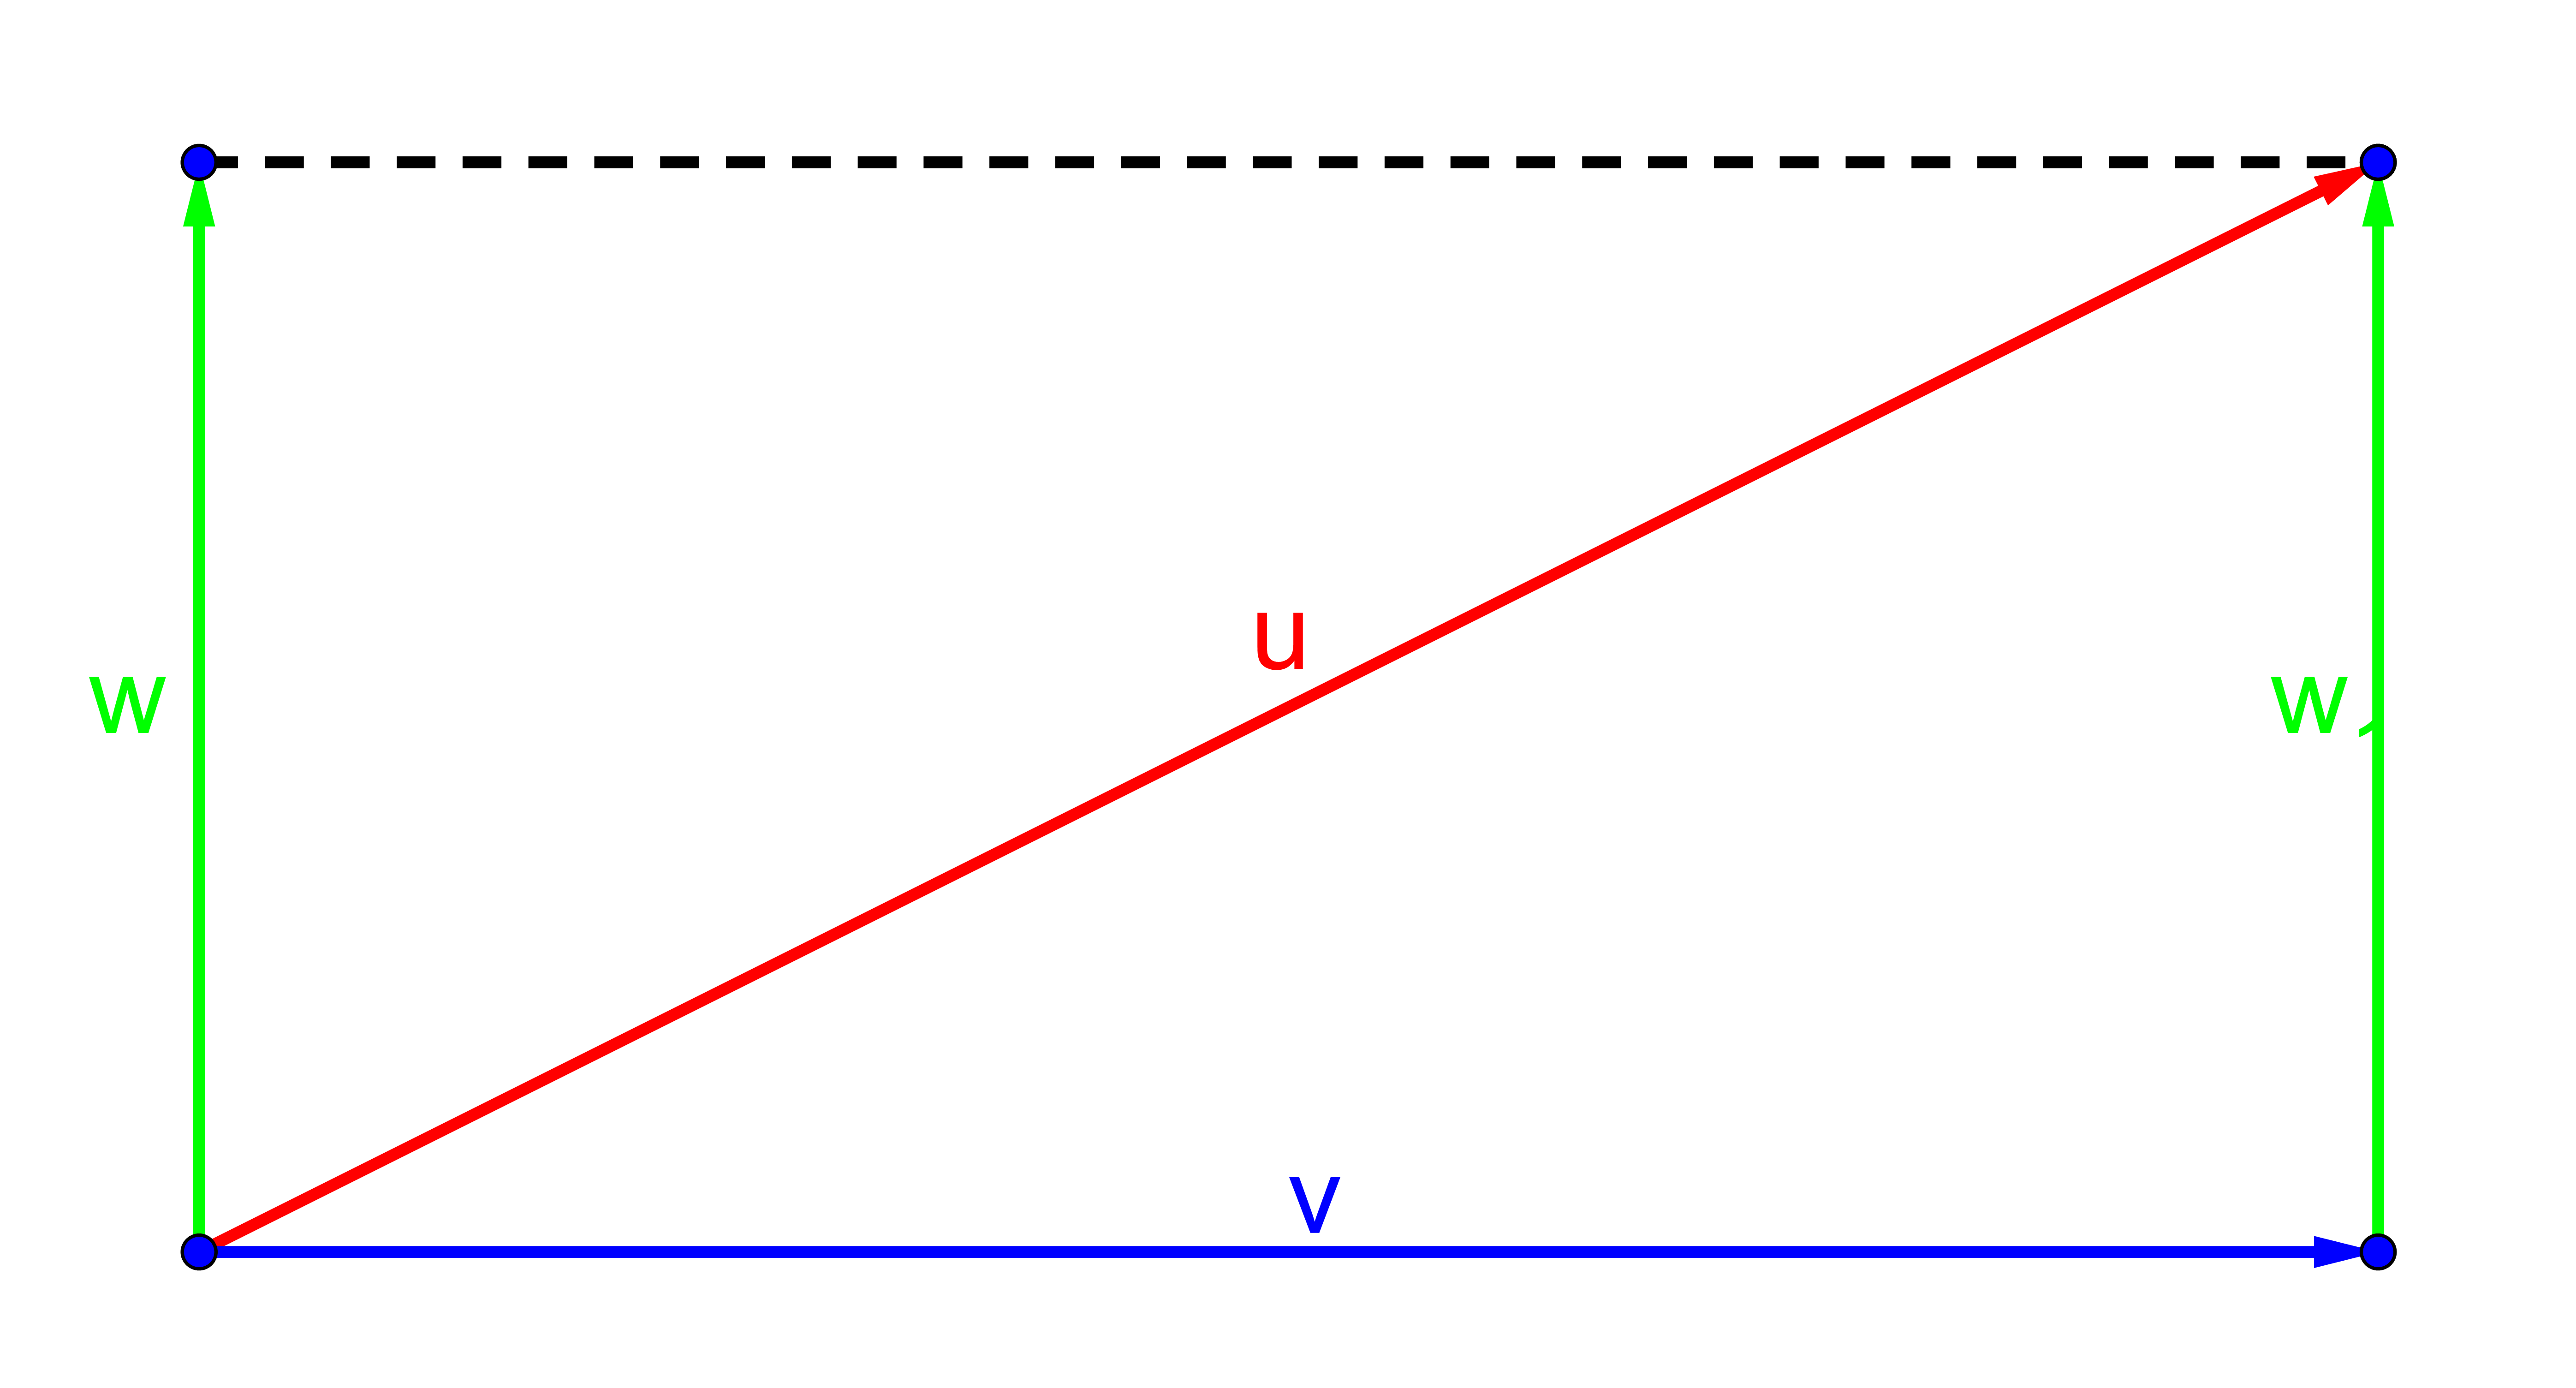
\includegraphics[width=3cm]{pythogorean.png}
  		\label{py} 
  	}
  	\subfigure{
  		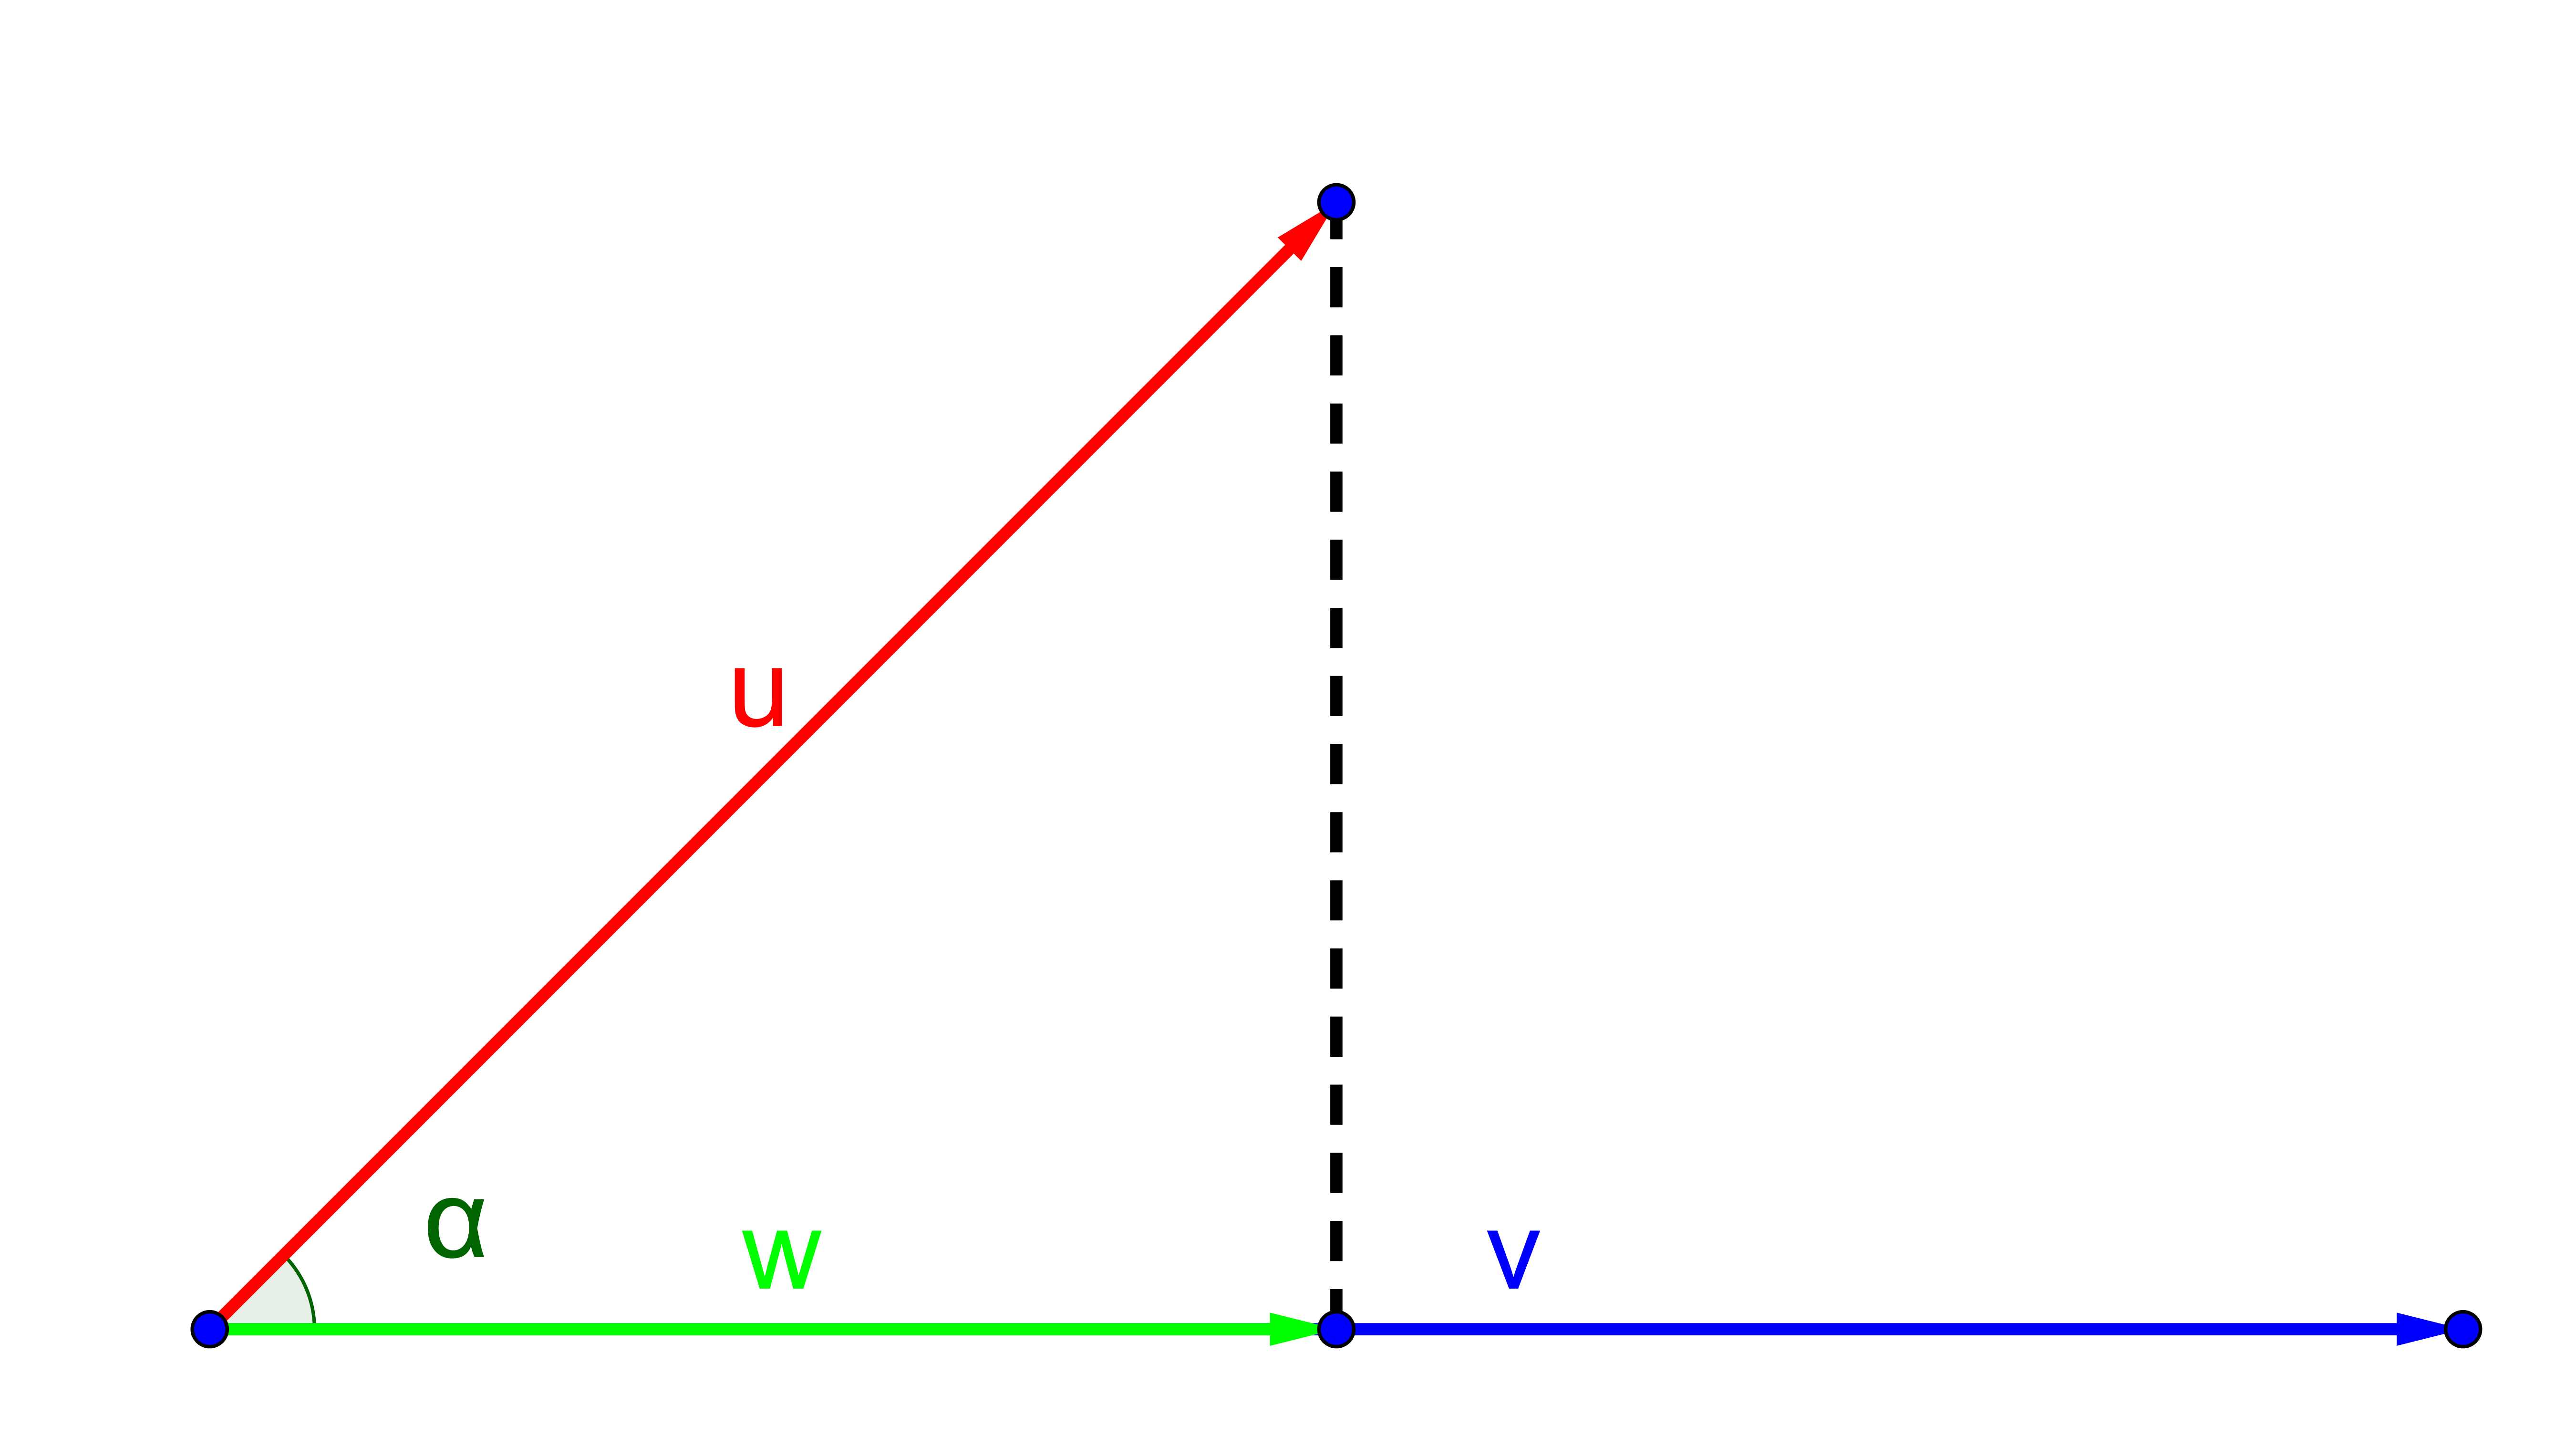
\includegraphics[width=3cm]{projection2.png}
  		\label{In}
  	}
  	\subfigure{
  		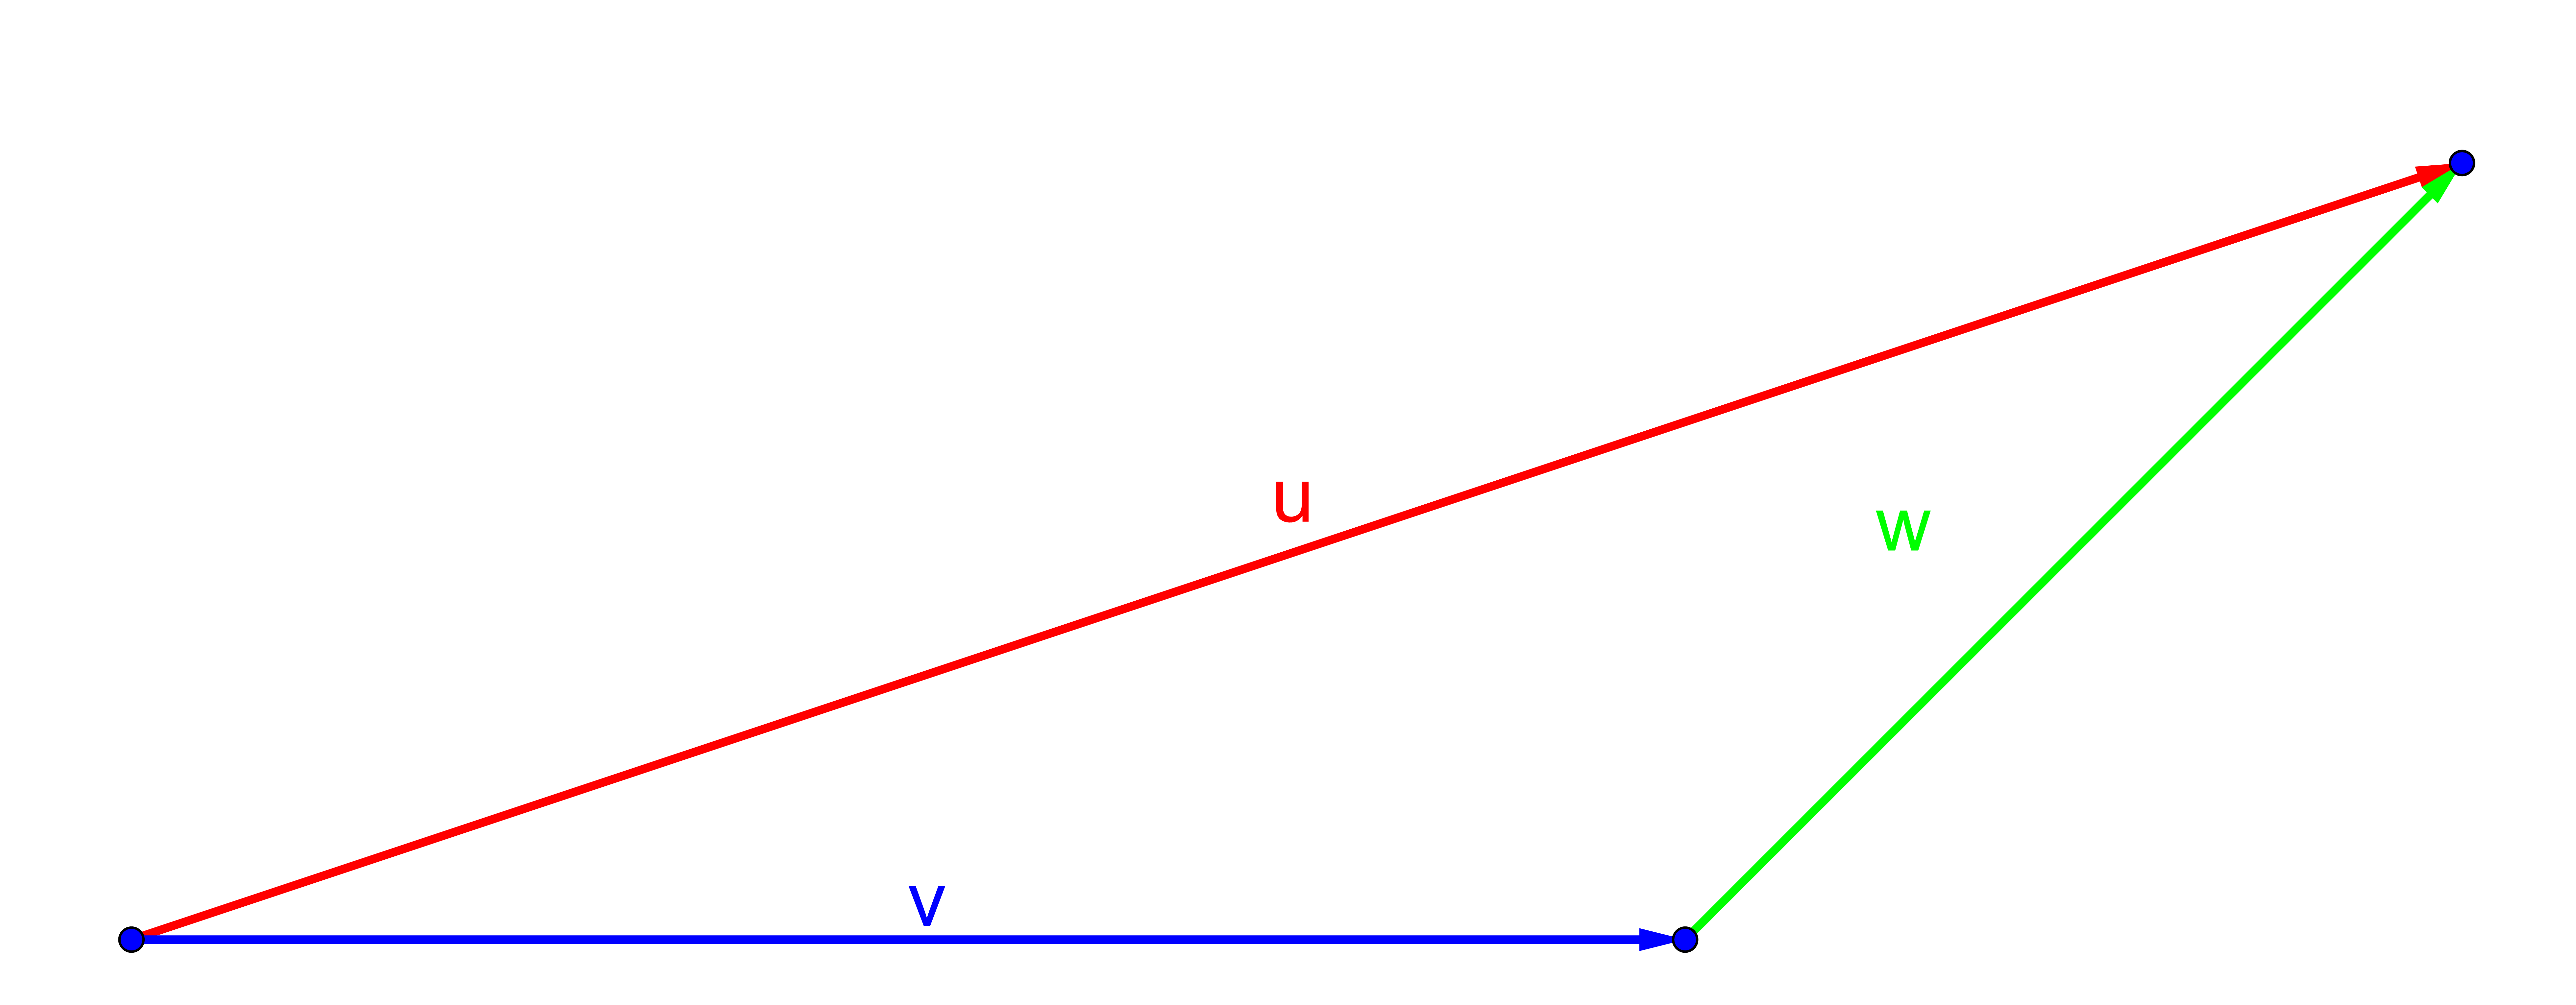
\includegraphics[width=3cm]{triangle.png}
  		\label{tri}
  	}
  	\caption{不等式}
  	\label{transformation}
  \end{figure}
\end{frame}
\begin{frame}[fragile]{集合的正交}
	\setbeamertemplate{description item}[align left]
	設$S=\left\{v_{1} ,v_{2} \cdots ,v_{n} \right\}$,$\forall i,v_{i} \ne 0$\\
	\begin{description}
		\item[正交集(orthogonal set)] \hfill \\若對於任意$i\ne j$有$v_{i} \cdot v_{j} =0$,則$S$為正交集合
		\item[正交規範集(orthonormal set)] \hfill \\
		若$S$為正交集且$\left\| v_{i} \right\| =1$,則$S$為正交規範集
	\end{description}
\end{frame}


\section{Gram Schimidt過程}

\begin{frame}{目標}
	希望將一個子空間的基底轉換成正交基底,方便映射與計算長度。因此我們的問題是:
	\begin{itemize}
		\item 可以將一個基底轉成正交基底嗎?
		\item 如果可以怎麼轉?
	\end{itemize}
	
\end{frame}

\begin{frame}{Gram Schimidt過程}
	考慮$\mathrm{\{}$$S=\left\{u_{1} ,u_{2} ,\cdots ,u_{n} \right\}$為一基底,令:\[\begin{array}{l} {v_{1} =u_{1} } \\ {v_{2} =u_{2} -\frac{u_{2} \cdot v_{1} }{\left\| v_{1} \right\| ^{2} } v_{1} } \\ {\qquad \vdots } \\ {v_{i} =u_{i} -\frac{u_{i} \cdot v_{1} }{\left\| v_{1} \right\| ^{2} } v_{1} -\frac{u_{i} \cdot v_{2} }{\left\| v_{2} \right\| ^{2} } v_{2} \cdots -\frac{u_{i} \cdot v_{i{\rm -1}} }{\left\| v_{i{\rm -1}} \right\| ^{2} } v_{i{\rm -1}} } \\ {\qquad \vdots } \end{array}\] 
	則$S{'} =\left\{v_{1} ,v_{2} ,\cdots ,v_{n} \right\}$為一正交基底。
	
\end{frame}
\begin{frame}[fragile]{性質}
	設$S$為一正交集,則$S$線性獨立。
	\begin{figure}[H]
		\centering
		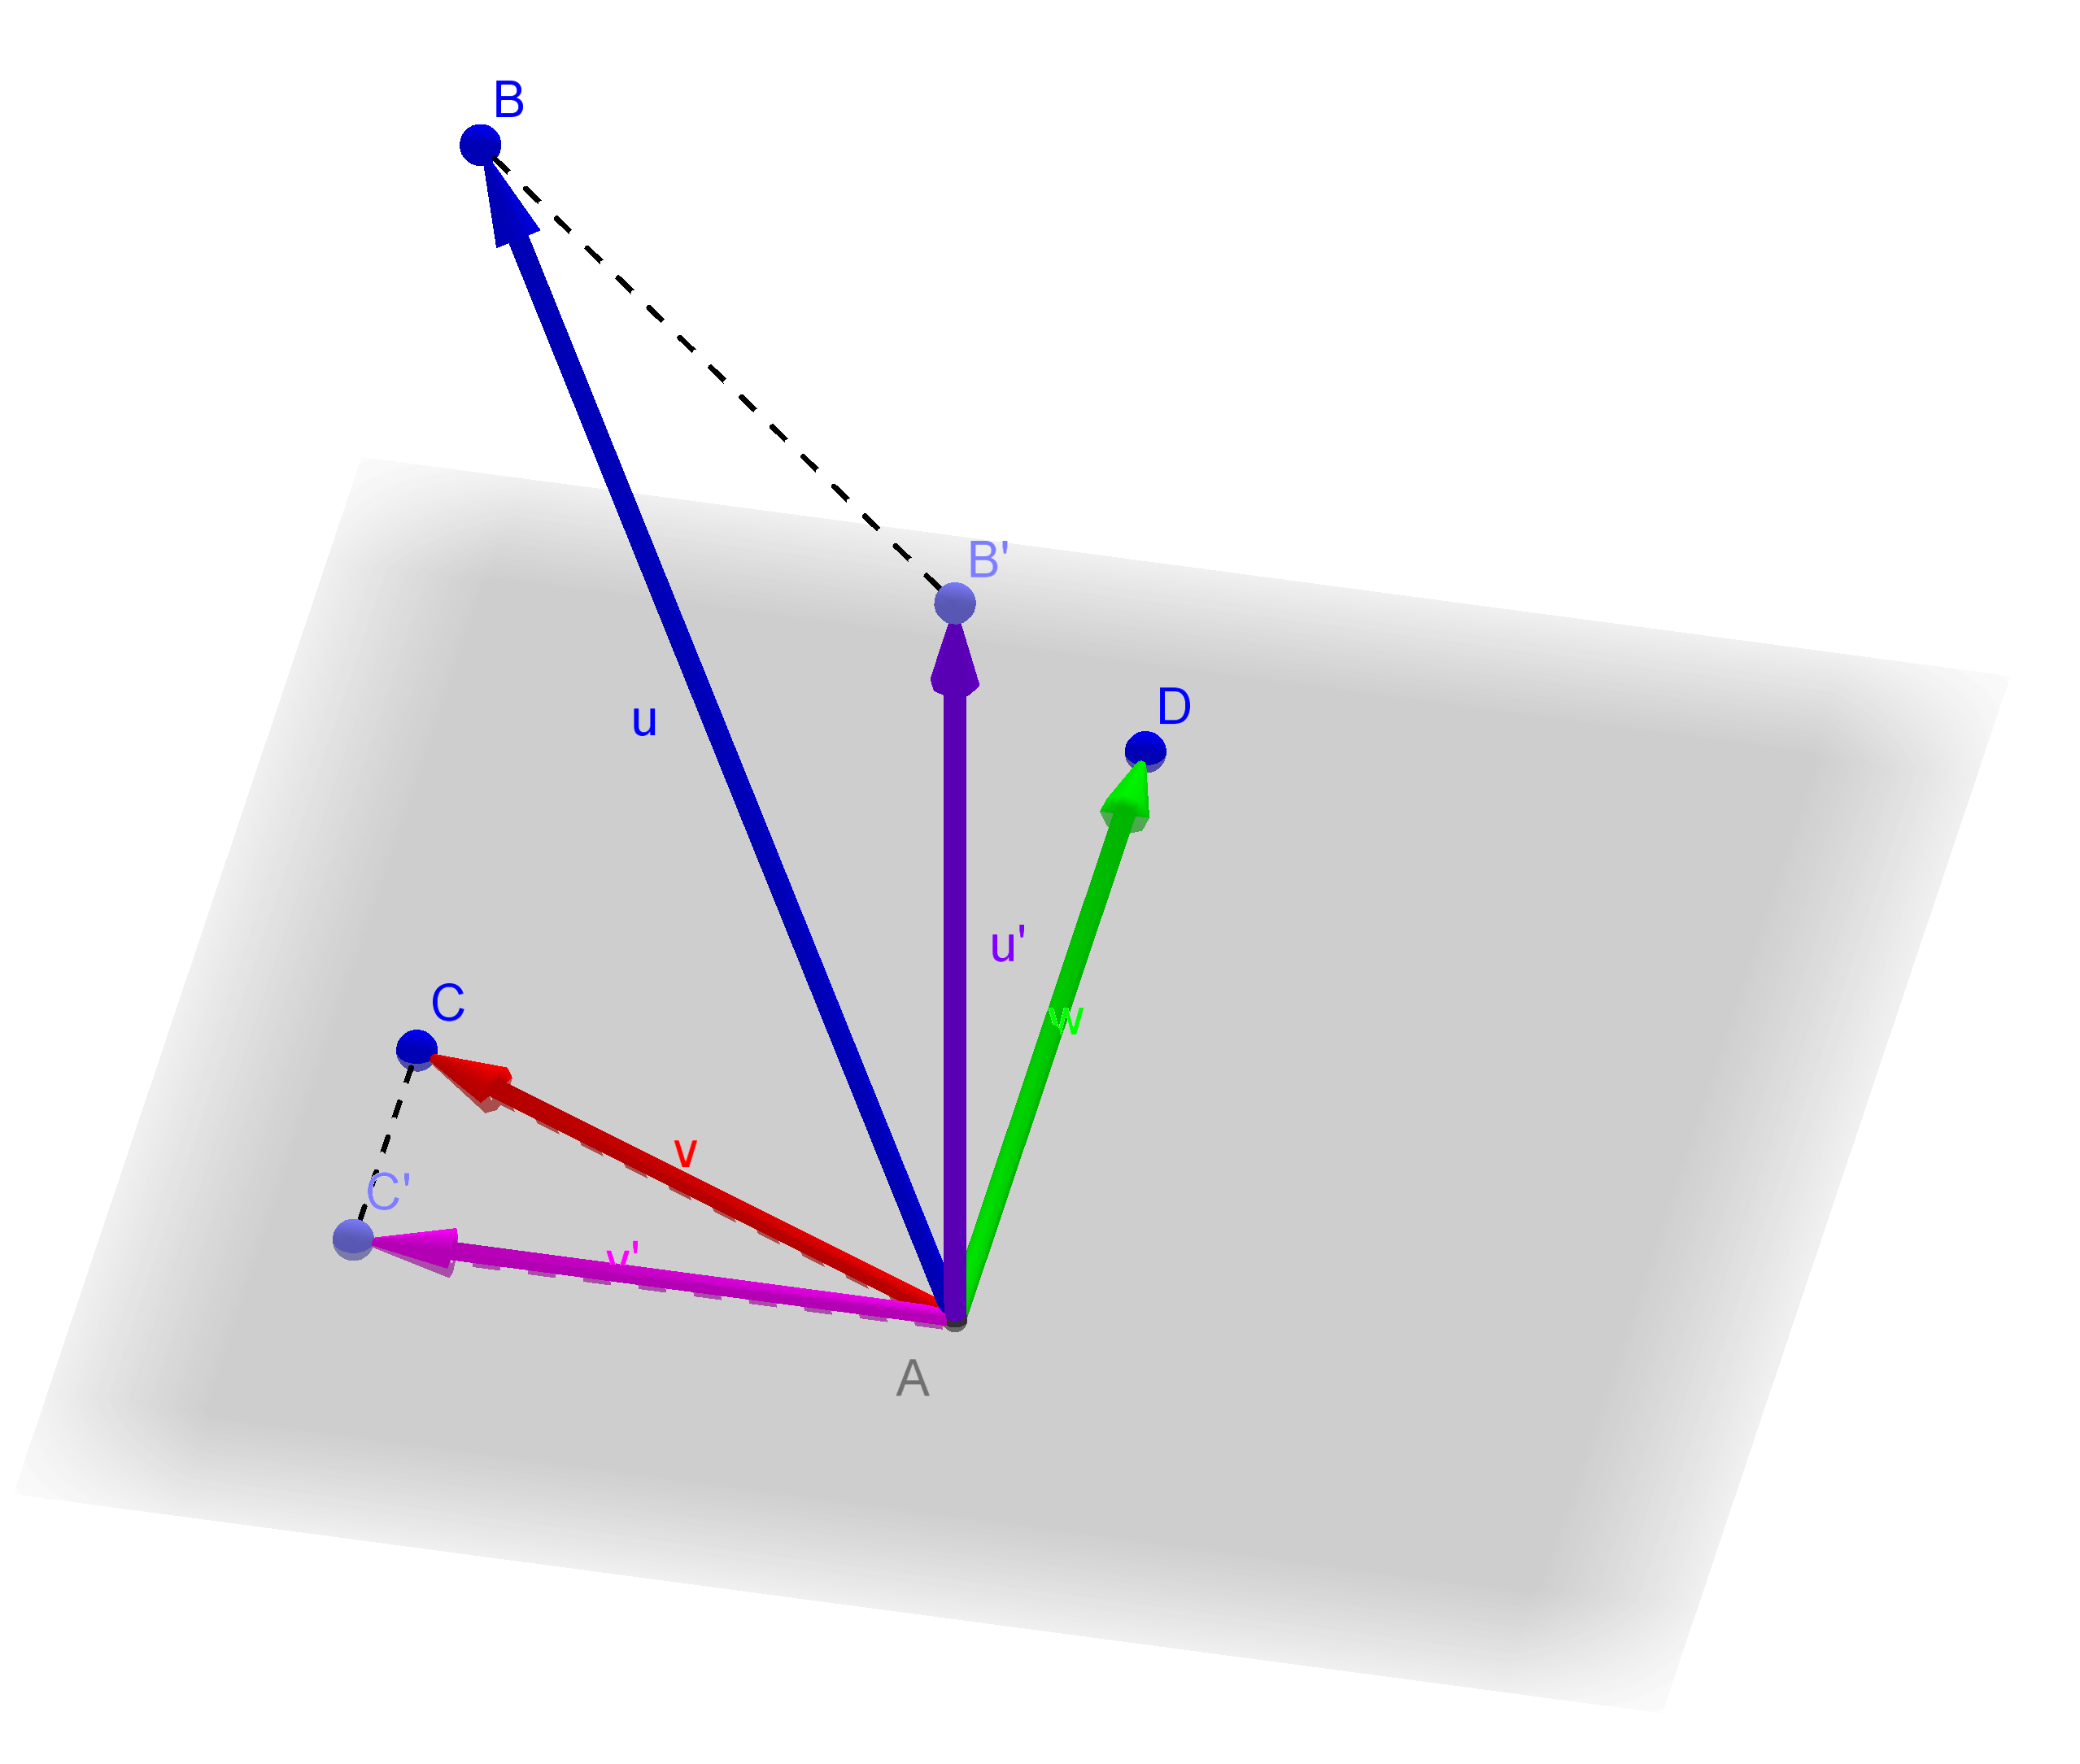
\includegraphics[height=5cm]{gramschmidt.png}
		\caption{圖像化}
		\label{fig:gram-schmidt}
	\end{figure}
\end{frame}

\begin{frame}{正交補餘 Orthogonal Complement}
	\begin{alertblock}{定義}
		非空集合$S$的正交補餘定義為
		\begin{equation*}
		S^{\bot } =\left\{v\in {\rm R}^{n} :u\cdot v=0,\forall u\in S\right\} 
		\end{equation*}
	\end{alertblock}
	\begin{exampleblock}{意義}
		非空集合$S$為矩陣$A$的列空間,則其正交補餘為$A$的零空間。
	\end{exampleblock}
\end{frame}
\begin{frame}{正交投影 Orthogonal Projection}
	\begin{alertblock}{定義}
		令$W\subset {\rm R}^{n} $,對於$v\in {\rm R}^{n} $存在的唯一向量$w\in W$有$\left(v-w\right)\in W^{\perp}$ ,則稱$w$為$v$的正交投影,並可定義運算子$P:{\rm R}^{n} \rightarrow W$,$P(v)=w\in W^ \perp$
		\begin{exampleblock}{問題}
			給定一子空間$W\subset {\rm R}^n$,要怎麼找到任意向量$v\in {\rm R}^n$的正交投影?\\
			如果是正交規範基底,問題會不會比較簡單?
		\end{exampleblock}
	\end{alertblock}	
\end{frame}
\begin{frame}{正交投影 Orthogonal Projection}
	\begin{figure}[H]
		\centering
		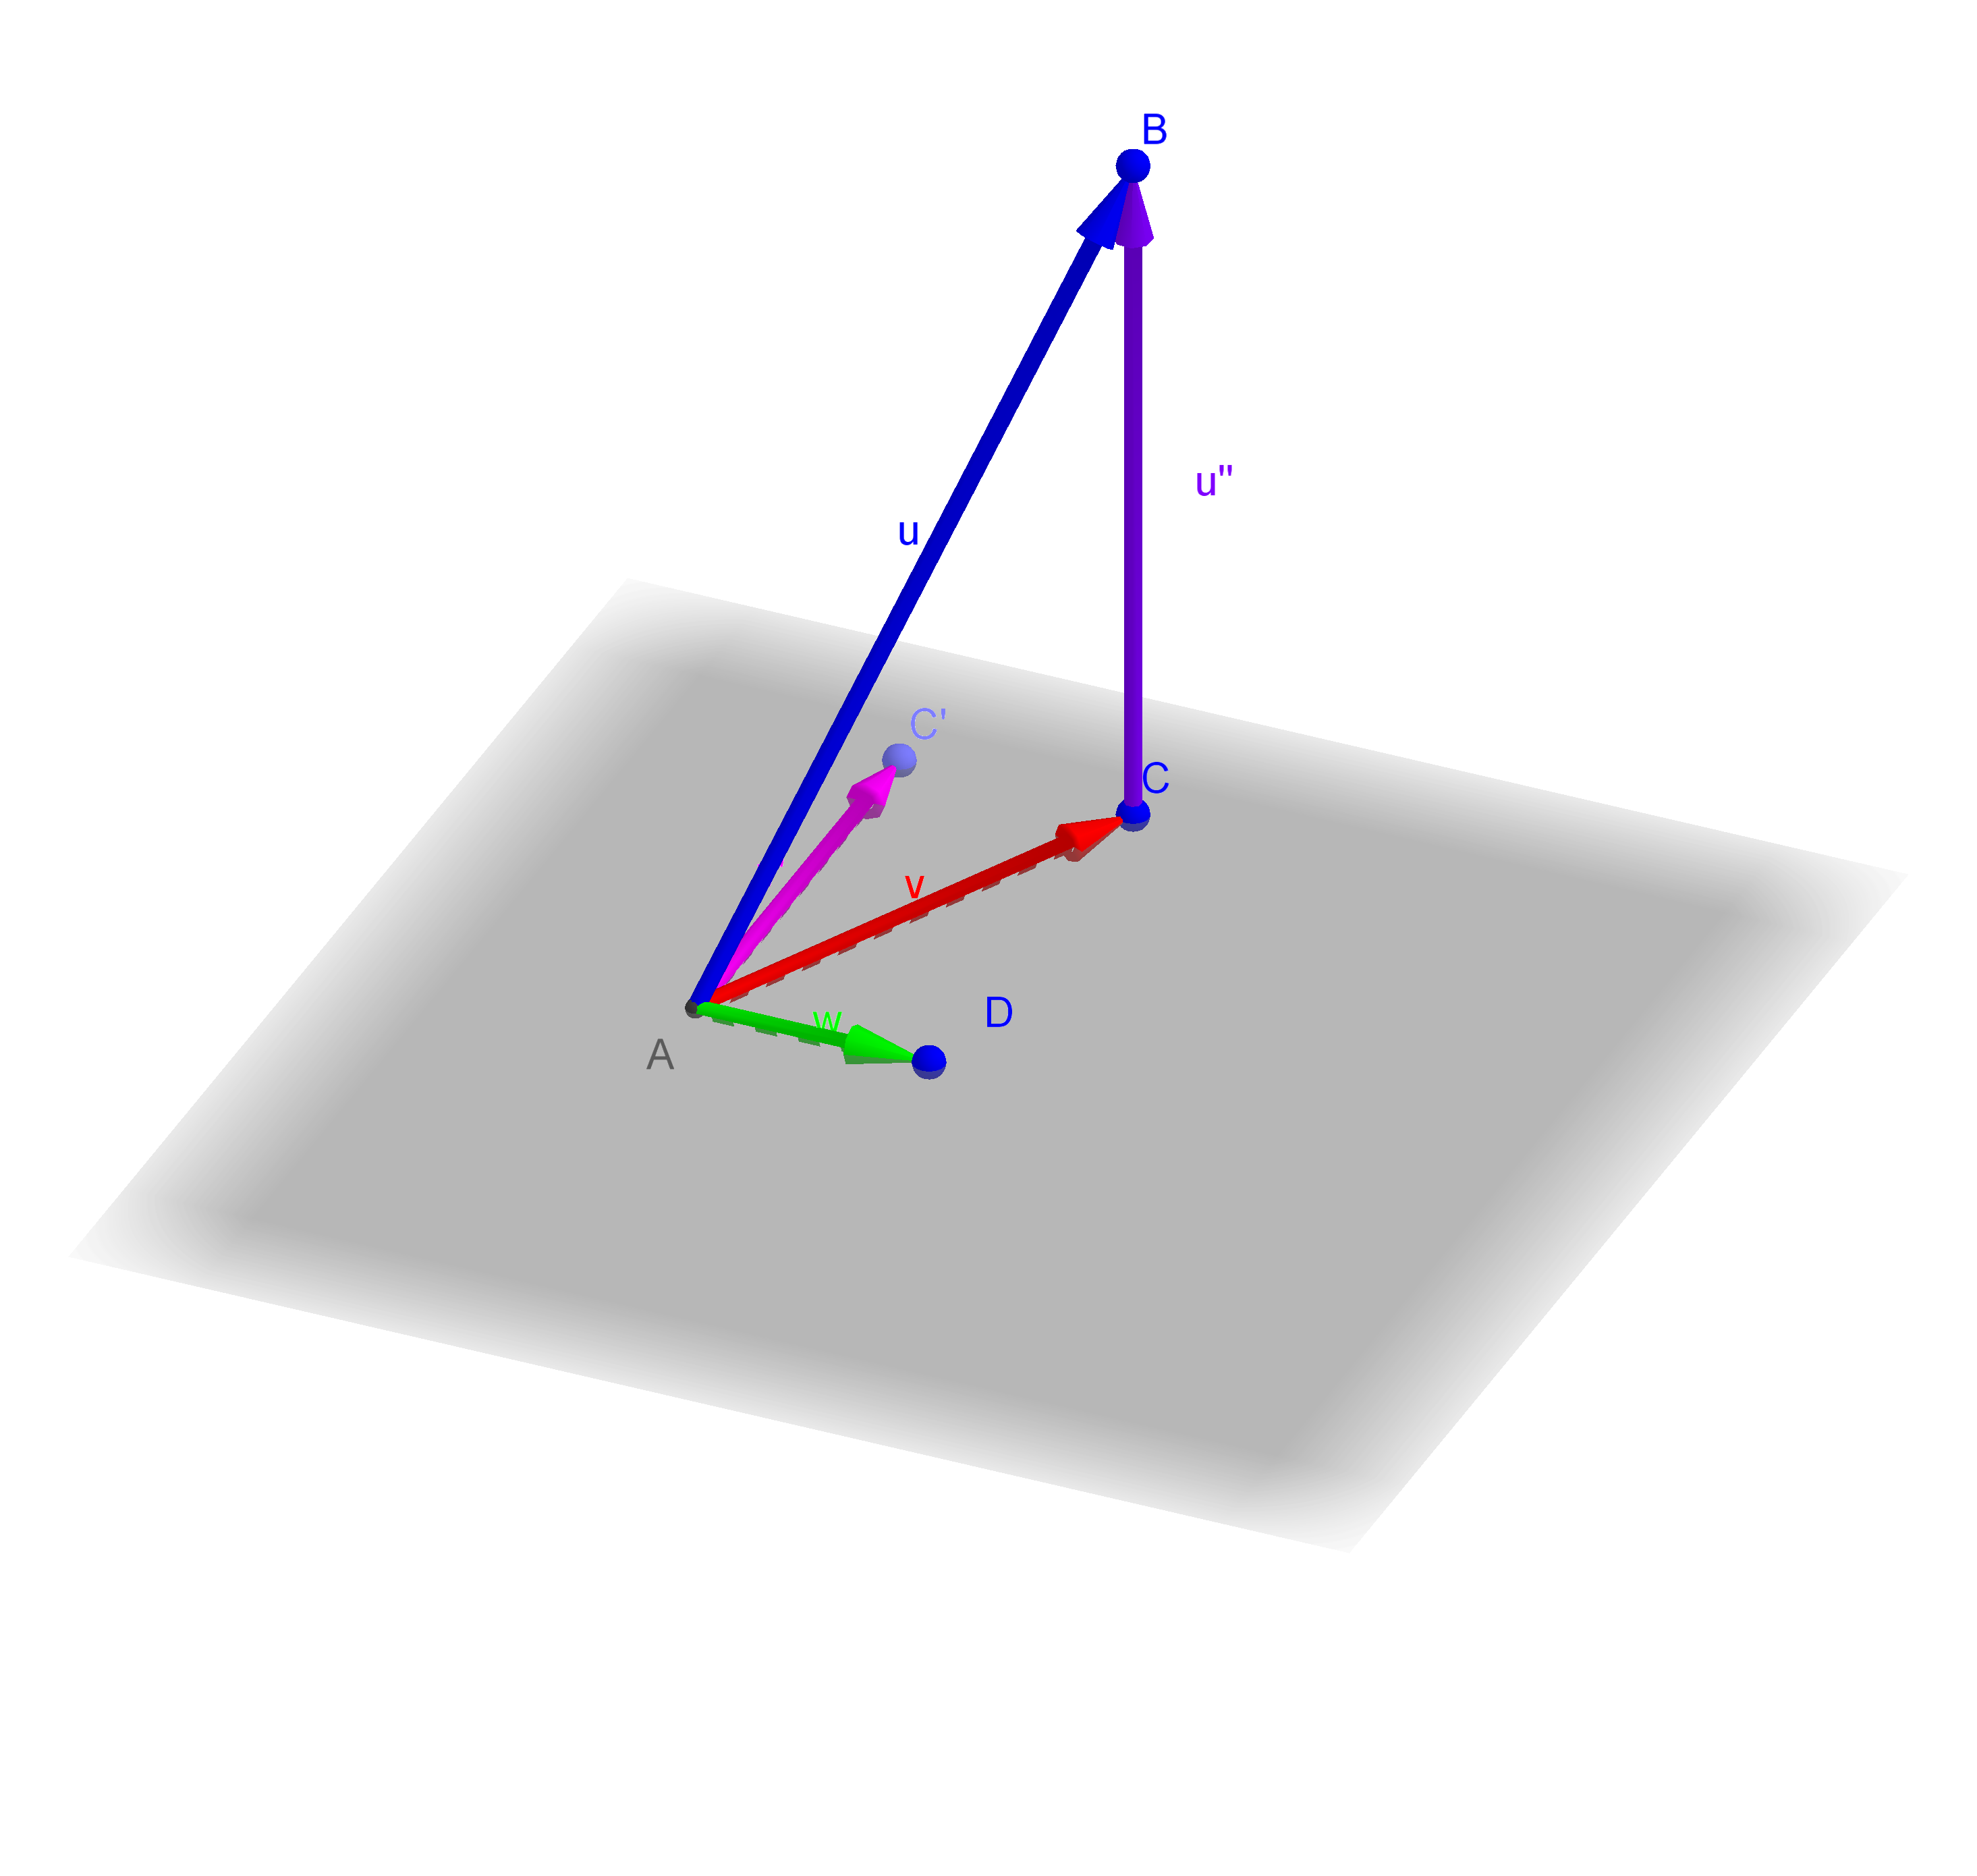
\includegraphics[height=6cm]{orthogonalprojection.png}
		\caption{圖像化}
		\label{fig:orthogonal-projection}
	\end{figure}	
\end{frame}
\begin{frame}{正交規範基底 Orthonormal Basis}
	令$\displaystyle W=\left\{ {{{z}_{1}},{{z}_{2}},\cdots ,{{z}_{n}}} \right\}$為正交規範基底。
	
	對於$v\in {{\rm{R}}^{n}}$,$v=w+u,w\in W,u\in {{W}^{\bot }}$,考慮:
	\[w=({{v}^{T}}{{z}_{1}}){{z}_{1}}+({{v}^{T}}{{z}_{2}}){{z}_{2}}+\cdots +({{v}^{T}}{{z}_{2}}){{z}_{2}}\]
	對於任意${{z}_{i}}\in Z$:
	\begin{align*}
	 & {{z}_{i}}^{T}(v-w)\\
	 = & {{z}_{i}}^{T}(v-({{v}^{T}}{{z}_{1}}){{z}_{1}}-({{v}^{T}}{{z}_{2}}){{z}_{2}}-\cdots -({{v}^{T}}{{z}_{2}}){{z}_{2}}) \\ 
	 = & {{z}_{i}}^{T}v-({{v}_{i}}^{T}{{z}_{i}})({{z}_{i}}^{T}{{z}_{i}}) \\ 
	 = & 0  
	\end{align*}
	\begin{exampleblock}{問題}
		如果是任意的基底呢?
	\end{exampleblock}
\end{frame}
\begin{frame}{正交規範基底}
	故$(v-w)\in {{W}^{\bot }}$,故$w$是$v$的正交投影。\\
	\begin{align*}
	w=&\left[ \begin{matrix}
	{{z}_{1}} & {{z}_{2}} & \cdots  & {{z}_{n}}  \\
	\end{matrix} \right]\left[ \begin{matrix}
	{{z}_{1}}^{T}v  \\
	{{z}_{2}}^{T}v  \\
	\vdots   \\
	{{z}_{n}}^{T}v  \\
	\end{matrix} \right]\\
	=&\left[ \begin{matrix}
	{{z}_{1}} & {{z}_{2}} & \cdots  & {{z}_{n}}  \\
	\end{matrix} \right]\left[ \begin{matrix}
	{{z}_{1}}^{T}  \\
	{{z}_{2}}^{T}  \\
	\vdots   \\
	{{z}_{n}}^{T}  \\
	\end{matrix} \right]v
	\end{align*}
 
	
\end{frame}
\begin{frame}{正交規範基底}
	\begin{figure}[H]
		\centering
		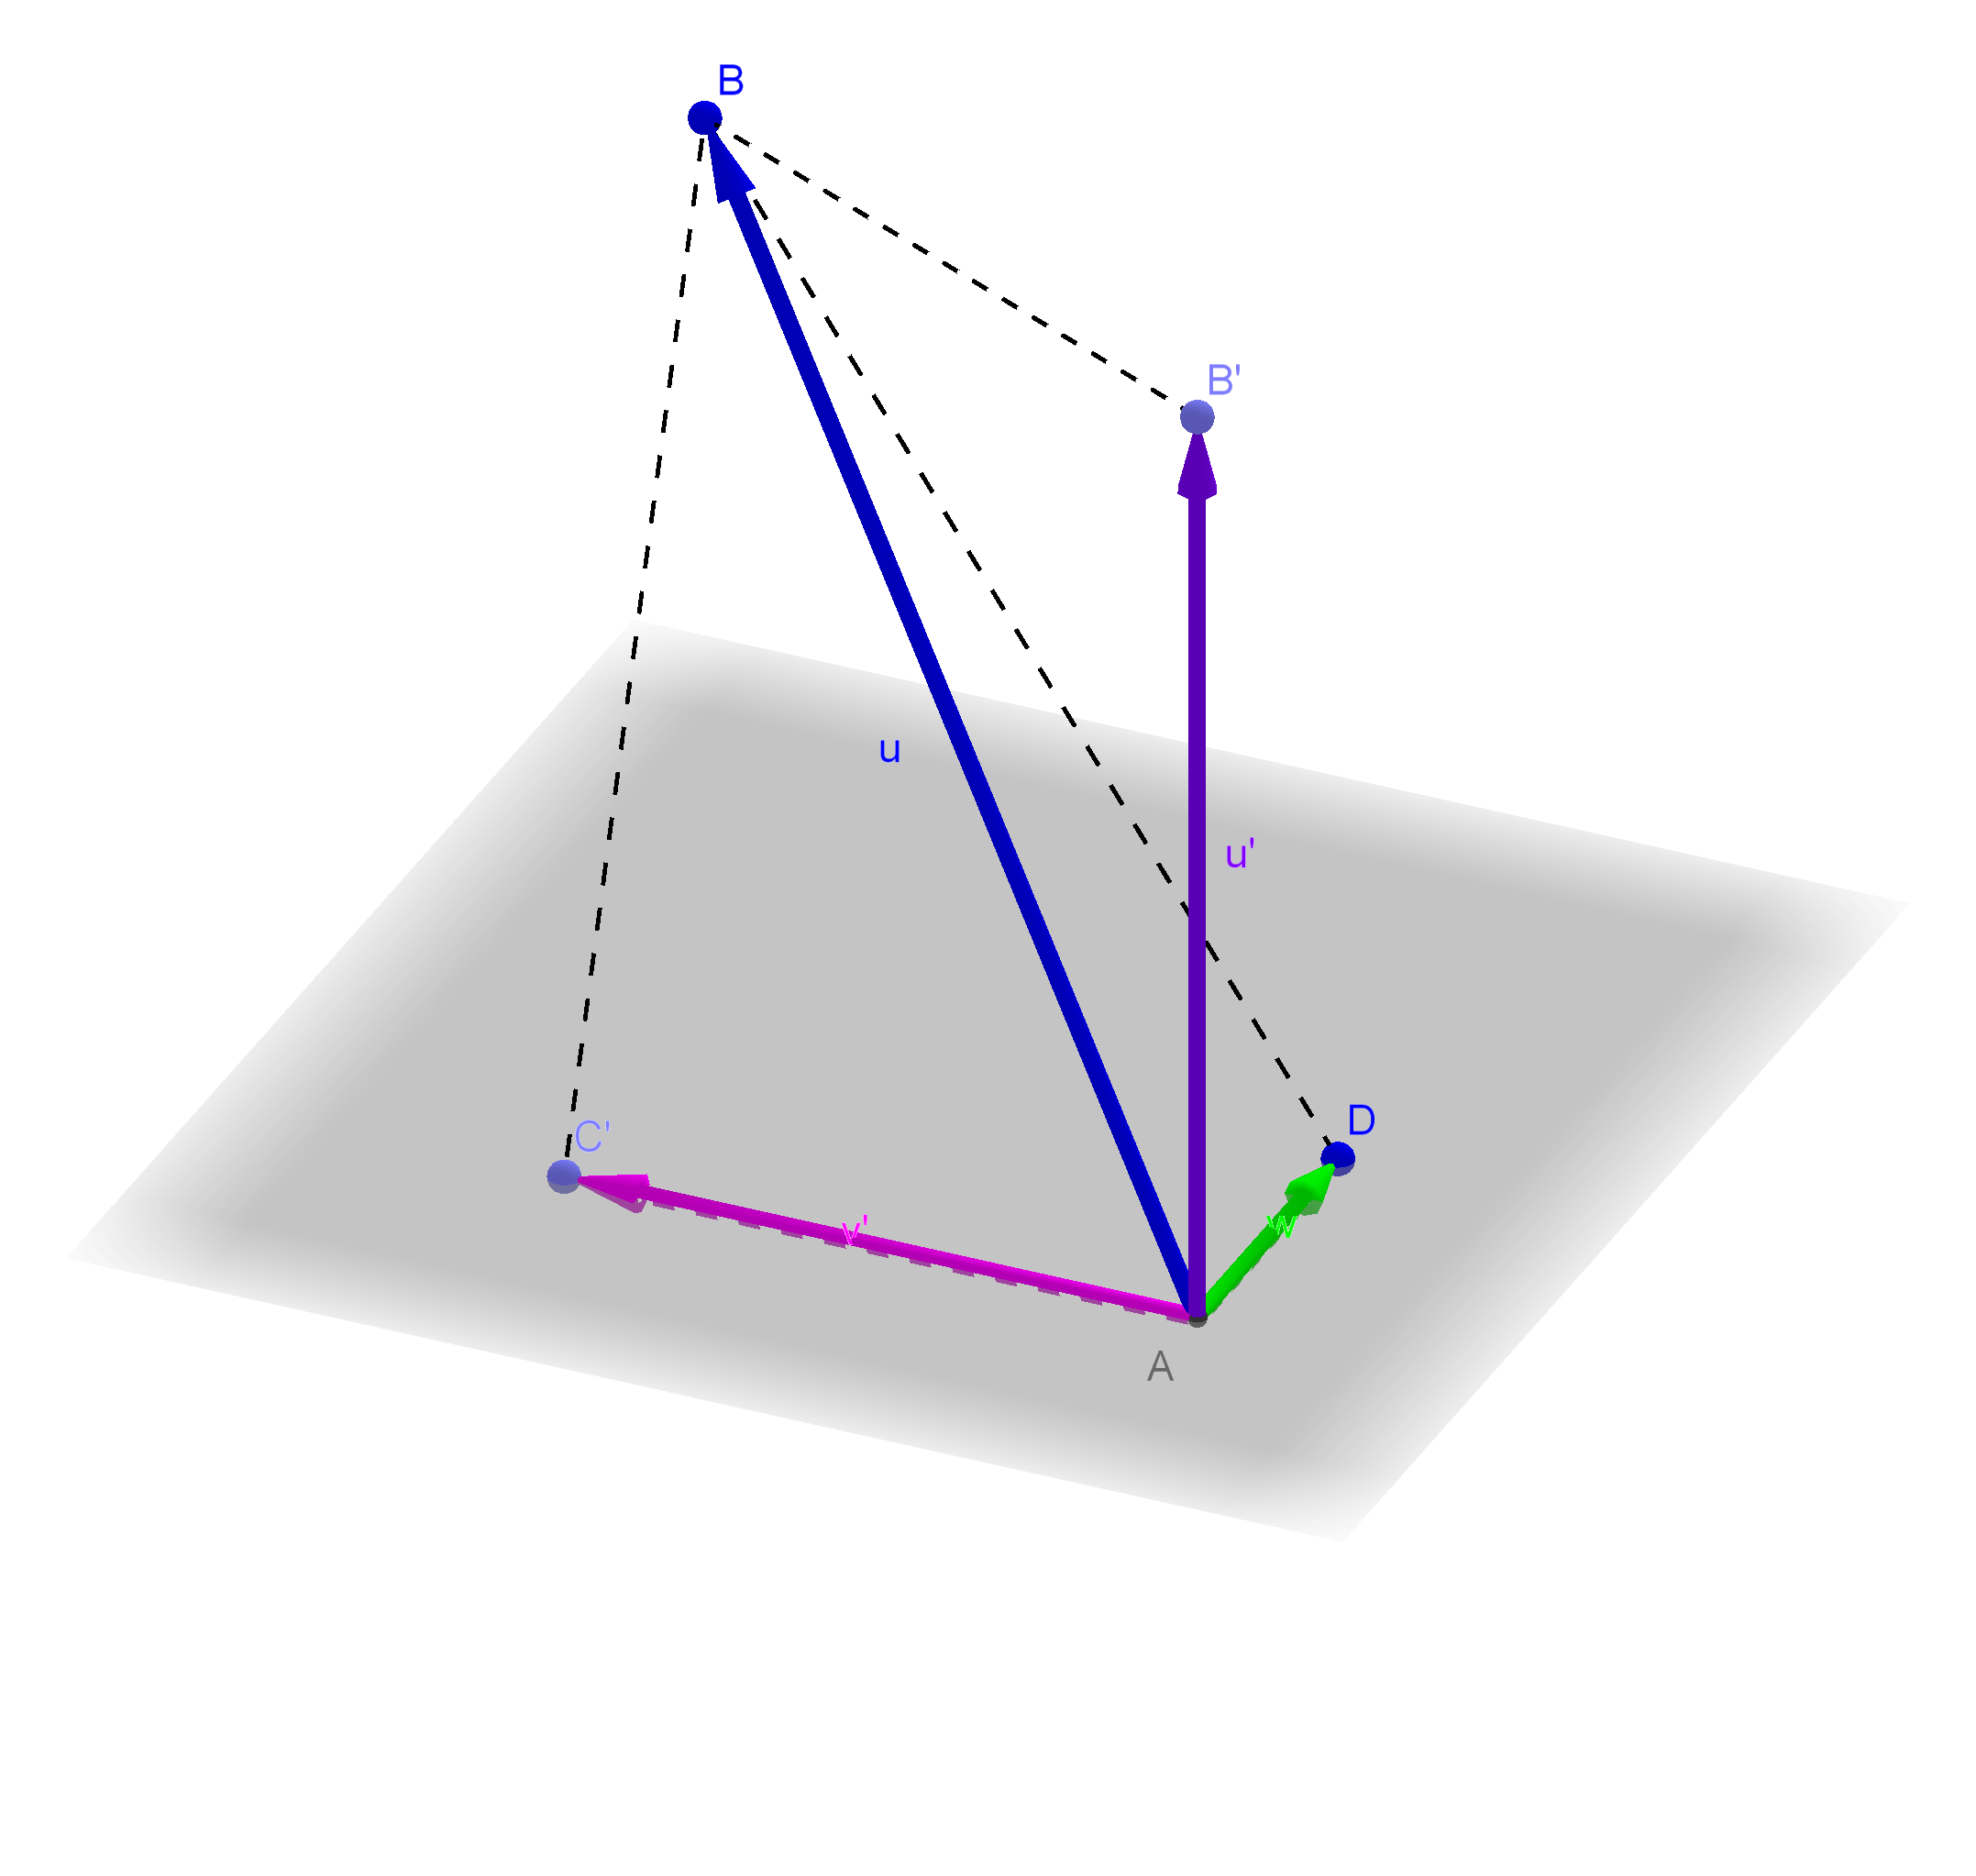
\includegraphics[height=6cm]{coordinate.png}
		\caption{圖像化}
		\label{fig:orthon}
	\end{figure}
\end{frame}
\begin{frame}{任意基底}
	設子空間$W\subset {{\rm{R}}^{n}}$的基底構成矩陣$A\in {{\rm{R}}^{m\times n}}$與\\
	設$w=Au\in W$為$v\in {{\rm{R}}^{n}}$的正交投影。考慮:
	\begin{align*}
	& {{W}^{\bot }}={{(\text{col }A)}^{\bot }}={{(\text{row }{{A}^{T}})}^{\bot }}=\text{null }{{A}^{T}} \\ 
	& \Rightarrow {{A}^{T}}(w-v)={{A}^{T}}Au-Av=0 \\ 
	& \Rightarrow {{A}^{T}}Au={{A}^{T}}v \\ 
	& \Rightarrow u={{({{A}^{T}}A)}^{-1}}{{A}^{T}}v \\ 
	& \Rightarrow w=Au=A{{({{A}^{T}}A)}^{-1}}{{A}^{T}}v \\ 
	\end{align*}
	
	
\end{frame}
\begin{frame}{任意基底}
	\begin{figure}[H]
		\centering
		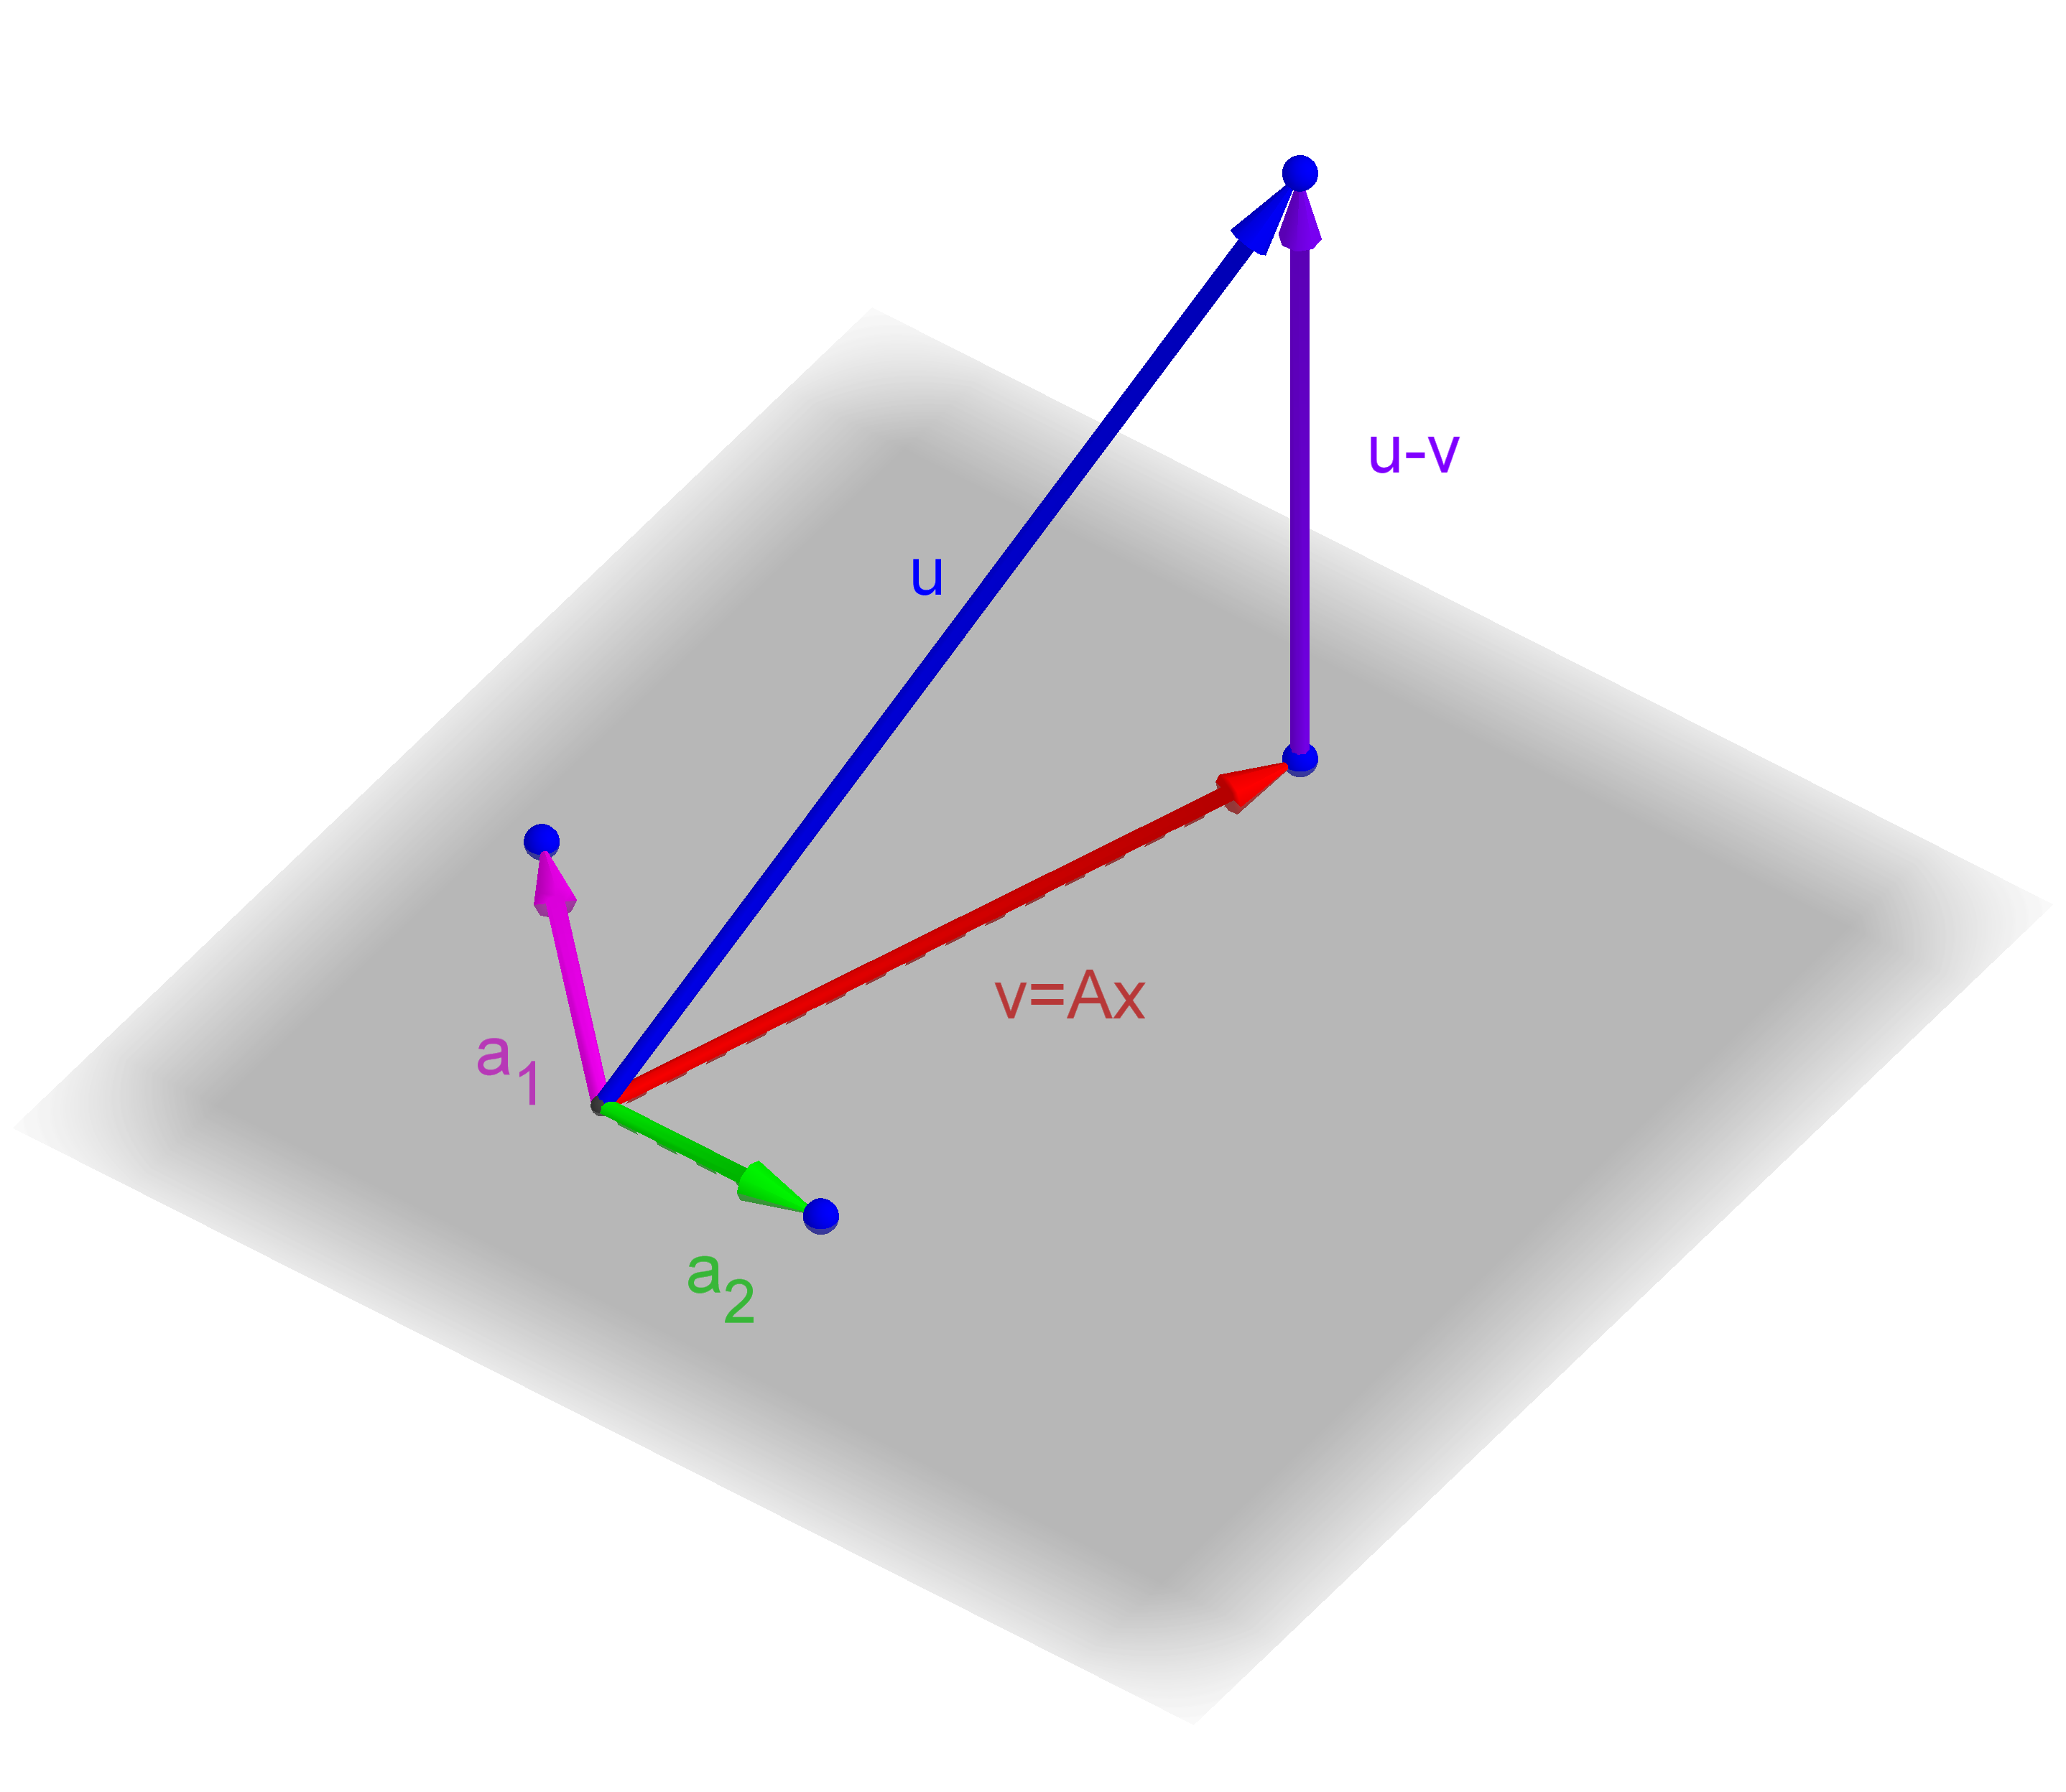
\includegraphics[height=6cm]{Pw.png}
		\caption{圖像化}
		\label{fig:any}
	\end{figure}
\end{frame}
\begin{frame}{正交矩陣 Orthogonal Matrix}
	\begin{alertblock}{定義}
		正交矩陣:若$Q$的行向量構成一{\color{red}正交規範基底},則$Q$為正交矩陣
	\end{alertblock}
	\begin{exampleblock}{定理}
		若且$Q\in {{\rm{R}}^{n\times n}}$,則:
		\begin{enumerate}
			\item ${{Q}^{T}}Q=I$$\Leftrightarrow$$Q$為正交矩陣 
			\item ${{(Qu)}^{T}}(Qv)={{u}^{T}}v$$\Leftrightarrow$$Q$為正交矩陣
		\end{enumerate}
	\end{exampleblock}
	
\end{frame}

\section{對稱矩陣與特徵空間}
\begin{frame}{對稱矩陣}
	\begin{exampleblock}{問題}
		為甚麼想找對稱矩陣?
	\end{exampleblock}
	因為對稱矩陣可以對角化,且其特徵向量相互正交。
\end{frame}
\begin{frame}{對稱矩陣 Symmetric Matrix}
	\begin{alertblock}{定義}
		對稱:若矩陣$A$有$A={{A}^{T}}$,則稱$A$對稱
	\end{alertblock}
	\begin{exampleblock}{定理}
		\begin{enumerate}
			\item 若$A=\left[ {{a}_{ij}} \right]\in {{\rm{R}}^{n\times n}},{{a}_{ij}}\in \rm{R},\forall i,j$,則${{f}_{A}}(t)=\det (A-t\cdot I)=0$有$n$實根。
			\item $A\in {{\rm{R}}^{n\times n}},A={{A}^{T}}$$\Leftrightarrow $存在正交矩陣$P$與對角矩陣$D$使$A=PD{{P}^{T}}$ 
		\end{enumerate}
	\end{exampleblock}
	
\end{frame}
\begin{frame}{光學分解 Spectral Decomposition}
	光學分解:考慮正交矩陣$P$與對角矩陣$D$使$A=PD{{P}^{T}}$,令:
	\[P=\left[ \begin{matrix}
	{{v}_{1}} & {{v}_{2}} & \cdots  & {{v}_{n}}  \\
	\end{matrix} \right],D=\left[ \begin{matrix}
	{{\lambda }_{1}} & 0 & \cdots  & 0  \\
	0 & {{\lambda }_{2}} & {} & \vdots   \\
	\vdots  & {} & \ddots  & 0  \\
	0 & \cdots  & 0 & {{\lambda }_{n}}  \\
	\end{matrix} \right]\]
	則:
	\[A={{\lambda }_{1}}{{v}_{1}}{{v}_{1}}^{T}+{{\lambda }_{2}}{{v}_{2}}{{v}_{2}}^{T}+\cdots +{{\lambda }_{n}}{{v}_{n}}{{v}_{n}}^{T}\] 
\end{frame}
\begin{frame}{問題}
	\begin{exampleblock}{問題}
		\begin{enumerate}
			\item {\bf 為甚麼要考慮對稱矩陣?}\\ 對稱矩陣可以對角化,且其不同特徵空間的向量相互正交。\\
			\item {\bf 為甚麼要考慮特徵空間?}\\	特徵值可以告訴我們長度的變化。\\
			\item {\bf 考慮許多線性變換的矩陣表達式不是對稱矩陣,想了解它的特徵空間有什麼方法?}\\ 考慮SVD!\\
		\end{enumerate}
	\end{exampleblock}
\end{frame}
\begin{frame}{什麼是對角化?}
	如果把矩陣$A$想像成一個函數,且$A$可以寫成$A=PDP^{-1}$,則:
	\[
	Av=\underbrace{P}_{\text{映射回$A$的空間}}\hspace{0.6cm}\underbrace{D}_{\text{縮放}}\hspace{1cm}\underbrace{{{P}^{-1}}}_{\text{取座標}}v
	\]
	 
\end{frame}
\begin{frame}{SVD是什麼?}
	\begin{figure}[H]
		\centering
		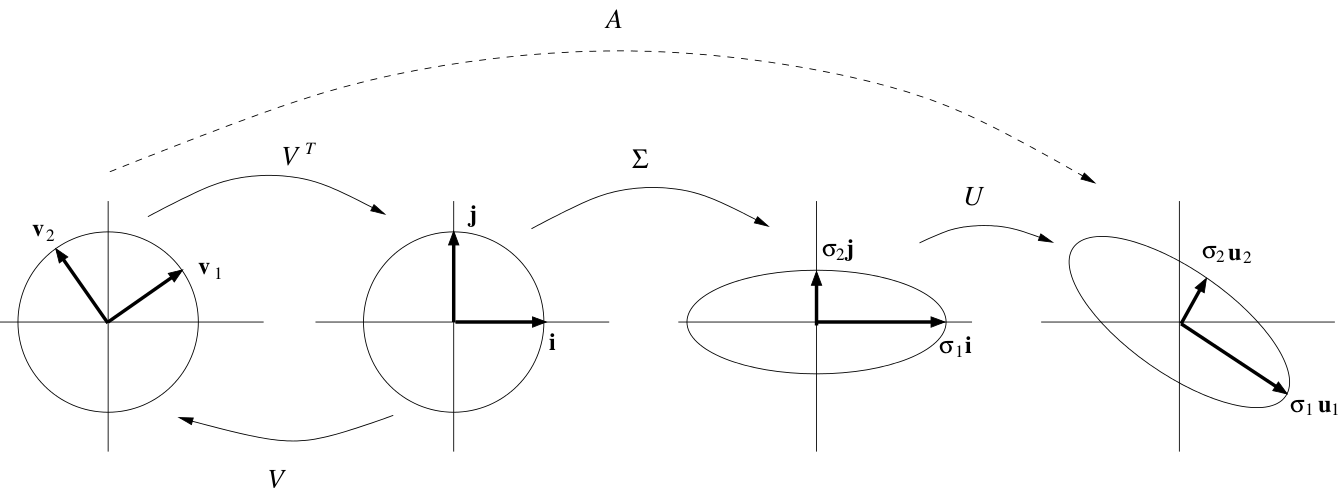
\includegraphics[width=10cm]{SVD1.png}
		\caption{圖像化}
		\label{fig:SVD}
	\end{figure}
\end{frame}
\begin{frame}{Singular Value Decomposition (SVD)}
	\begin{exampleblock}{定理}
		設$A\in {{\rm{R}}^{m\times n}}$,$\text{Rank }A=k$,則存在${{\rm{R}}^{n}}$的正交規範基底$\left\{ {{v}_{1}},{{v}_{2}},\cdots ,{{v}_{n}} \right\}$與${{\rm{R}}^{m}}$的正交規範基底$\left\{ {{u}_{1}},{{u}_{2}},\cdots ,{{u}_{n}} \right\}$,以及${{\sigma }_{1}}\ge {{\sigma }_{2}}\ge \cdots \ge {{\sigma }_{k}}>0$,使得:
		\[A{{v}_{i}}=\left\{ \begin{array}{*{35}{l}}
		{{\sigma }_{i}}{{u}_{i}},1\le i\le k  \\
		0,i>k  \\
		\end{array} \right.,{{A}^{T}}{{u}_{i}}=\left\{ \begin{array}{*{35}{l}}
		{{\sigma }_{i}}{{v}_{i}},1\le i\le k  \\
		0,i>k  \\
		\end{array} \right.\]
	\end{exampleblock}
\end{frame}
\begin{frame}{Singular Value Decomposition (SVD)}
	\begin{figure}[H]
		\centering
		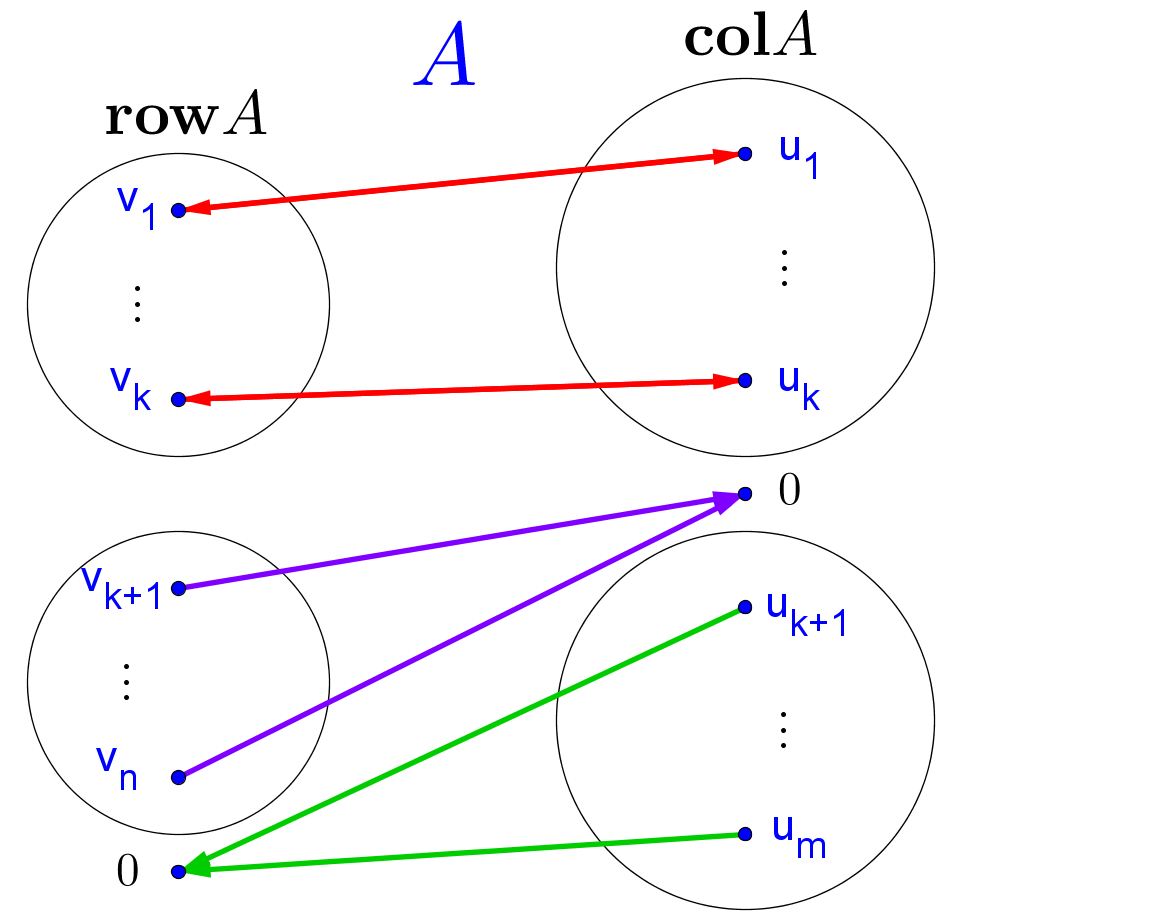
\includegraphics[height=6cm]{map.png}
		\caption{圖像化}
		\label{fig:SVDmap}
	\end{figure}
\end{frame}
\begin{frame}{問題}
	利用前頁的定理,令\\$V=\left[ \begin{matrix}
	{{v}_{1}} & {{v}_{2}} & \cdots  & {{v}_{n}}  \\
	\end{matrix} \right]$,\\$U=\left[ \begin{matrix}
	{{u}_{1}} & {{u}_{2}} & \cdots  & {{u}_{m}}  \\
	\end{matrix} \right]$,$\Sigma=[a_{ij}],{{a}_{ij}}=\left\{ \begin{array}{*{35}{l}}
	0,i\ne 0  \\
	{{\sigma }_{i}},i=j  \\
	\end{array} \right.
	$\\
	則:$AV= U\Sigma$\\
	或記為:$A= U\Sigma{}V^T$
	
	
\end{frame}

\begin{frame}[standout]
	Q\&A
\end{frame}
\begin{frame}[standout]
	謝謝大家
\end{frame}

\end{document}
